% - Tool di allineamento per la collazione:
%
% -- http://v-machine.org/documentation/
%
% -- https://collatex.net/
%
% -- http://www.juxtacommons.org/
%
% -- https://sada.uzi.uni-halle.de/
%
% -- medite
%
% -- tustep/TXSTEP
%
% -- stemmaWeb
%
% -- Classical Text Editor
%
% -- http://evt.labcd.unipi.it/

% -- http://www.informatik.uni-leipzig.de:8080/BibleViz/
% -- http://www.traviz.vizcovery.org/examples.html

% ecdotica: resa grafica, messa in pagina
% -- https://ride.i-d-e.de/issues/issue-11/reledmac/
% -- https://tei-c.org/2014/06/10/tei-critical-edition-toolbox/
% -- http://teicat.huma-num.fr/index.php

% Could be utilized to divide the process into an automated collation layer and a human interpretation layer.

\begin{frame}
	\frametitle{Strumenti per edizioni critiche}
	\addtocounter{nframe}{1}
    \begin{block}{processo automatizzabile}
       Le tecnologie digitali e i metodi computazionali stanno innovando il processo per lo studio e l'edizione dei testi.
    \end{block}
    \begin{block}{processo automatizzabile}
        Oggi è possibile dividere il processo di critica testuale in fasi sia sempre più automatizzabili (come la collazione) e in fasi interpretative/ermeneutiche saldamente nelle mani degli studiosi.
     \end{block}
	
\end{frame}

\begin{frame}
	\frametitle{Strumenti per edizioni critiche}
	\addtocounter{nframe}{1}
   
    \begin{center}
        \begin{itemize}
            \item Preparazione dell'edizione
            \item Visualizzazione e Pubblicazione dell'edizione
        \end{itemize}
    \end{center}
	
\end{frame}

\begin{frame}
	\frametitle{Strumenti per edizioni critiche}
	\addtocounter{nframe}{1}
    \begin{block}{Preparazione}
        Un filologo al fine di allestire un'edizione di un testo deve consultare - anche per tradizioni di medie grandezze e complessità - un gran numero di testimoni e di fonti secondarie/indirette. Di queste fonti lo studioso deve identificare, registrare e analizzare (quasi) tutte le differenze (varianti) presenti nel testo.
        
	\end{block}
	\begin{block}{Preparazione}
      E' possibile in tutto o in parte automatizzare qualche fase del processo di edizione? \textbf{Gestione dei testimoni? Collazione? Generazione Stemma Codicum? Codifica?}
	\end{block}
\end{frame}

%  Changes are catalogued in a critical apparatus
        % A typical entry starts with the variant’s position (usually line or paragraph number), followed by the lemma of the base text often delimited by a closing square bracket ‘]’
        % follows the variant text itself and finally the corresponding sigla of the sources
\begin{frame}
    \frametitle{Strumenti per edizioni critiche}
    \addtocounter{nframe}{1}
    
    \begin{block}{Visualizzazione}
        Non solo in fase di preparazione di una edizione le tecnologie digitali offrono supporto allo studioso, ma anche in fase di pubblicazione e di visualizzazione molte iniziative animano la comunità
    \end{block}
    
    \begin{block}{Visualizzazione}
        \begin{itemize}
            \item Visualizzare collazione tra testi
            \item Apparato critico dinamico
            \item Visualizzazione parallela di testi
        \end{itemize}
    \end{block}

\end{frame}

\begin{frame}
	\frametitle{Philological computational tools}
	\addtocounter{nframe}{1}
    \begin{block}{Collation tools}
            
        \begin{center}
            Tra gli strumenti più utili ai filologi ci sono quelli per la collazione automatica dei testi.

            % philological text collation tool needs to build a bridge between technical and scholarly understanding
            % Collating long texts turned out to be a complex scenario
            % 2009, a working group presented an abstract framework for complex text collation procedures, which was later called ‘Gothenburg mode
            % five different computing stages (tokenization, normalization, alignment, analysis, and visualization). Nassourou (2013) proposed to extend this model by a sixth, interpretative layer
		\end{center}
    \end{block}
    
    \begin{block}{Gothenburg Model}
        % 2009, a working group presented an abstract framework for complex text collation procedures, which was later called ‘Gothenburg mode
            % five different computing stages (tokenization, normalization, alignment, analysis, and visualization). Nassourou (2013) proposed to extend this model by a sixth, interpretative layer
            \begin{itemize}
                \item tokenization
                \item normalization
                \item alignment
                \item analysis
                \item visualization
                \item \textit{interpretative}
            \end{itemize}
    \end{block}
\end{frame}

\begin{frame}
	\frametitle{Philological computational tools}
	\addtocounter{nframe}{1}
    \begin{block}{Collation tools}
		\begin{itemize}
			\item CollateX
			\item Variance Viewer
			\item Juxta Web Service
			\item StemmaWeb
			\item TUSTEP/TXSTEP
			\item MEDITE
		\end{itemize}
	\end{block}
\end{frame}

\begin{frame}
	\frametitle{Philological computational tools}
	\addtocounter{nframe}{1}
    \begin{block}{Visualization/Publication tools}
		\begin{itemize}
			\item Classical Text Editor (CTE)
			\item TEIpublisher
			\item Edition Visualization Technology (EVT)
			\item TextualCommunities
			\item Versioning Machine
			\item LERA/SADA project
			\item Critical Edition Toolbox
			\item LaTex/Reledmac
			\item TRAVIZ/ITEAL
			\item EUPORIA
		\end{itemize}
	\end{block}
\end{frame}

% Stemma: si definisce stemma codicum o albero genealogico, la rappresentazione grafica dei rapporti genetici fra i testimoni, ricostruiti attraverso la rilevazione e la valutazione degli errori (vd.) di cui ciascuno è portatore.


\begin{frame}
    \frametitle{Strumenti per edizioni critiche}
    \framesubtitle{Strumenti di collazione automatica}
	\addtocounter{nframe}{1}
    \begin{center}
        \textbf{CollateX}
    \end{center}
    \begin{center}
        \textit{\url{https://collatex.net}}
	\end{center}
    \begin{center}
        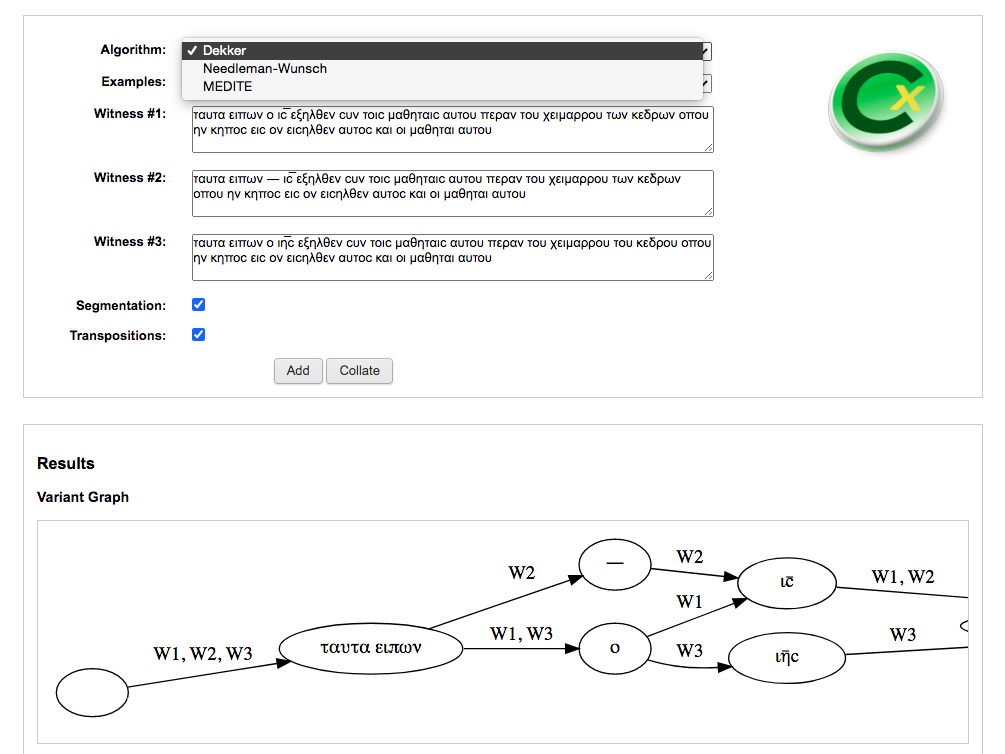
\includegraphics[width=.95\textwidth]{imgs/collatex.png}
	\end{center}
\end{frame}

\begin{frame}
    \frametitle{Strumenti per edizioni critiche}
    \framesubtitle{Strumenti di collazione automatica}
	\addtocounter{nframe}{1}
    \begin{center}
        \textbf{Variance Viewer}
    \end{center}
    \begin{center}
        \textit{\url{http://variance-viewer.informatik.uni-wuerzburg.de/Variance-Viewer/}}
	\end{center}
    \begin{center}
        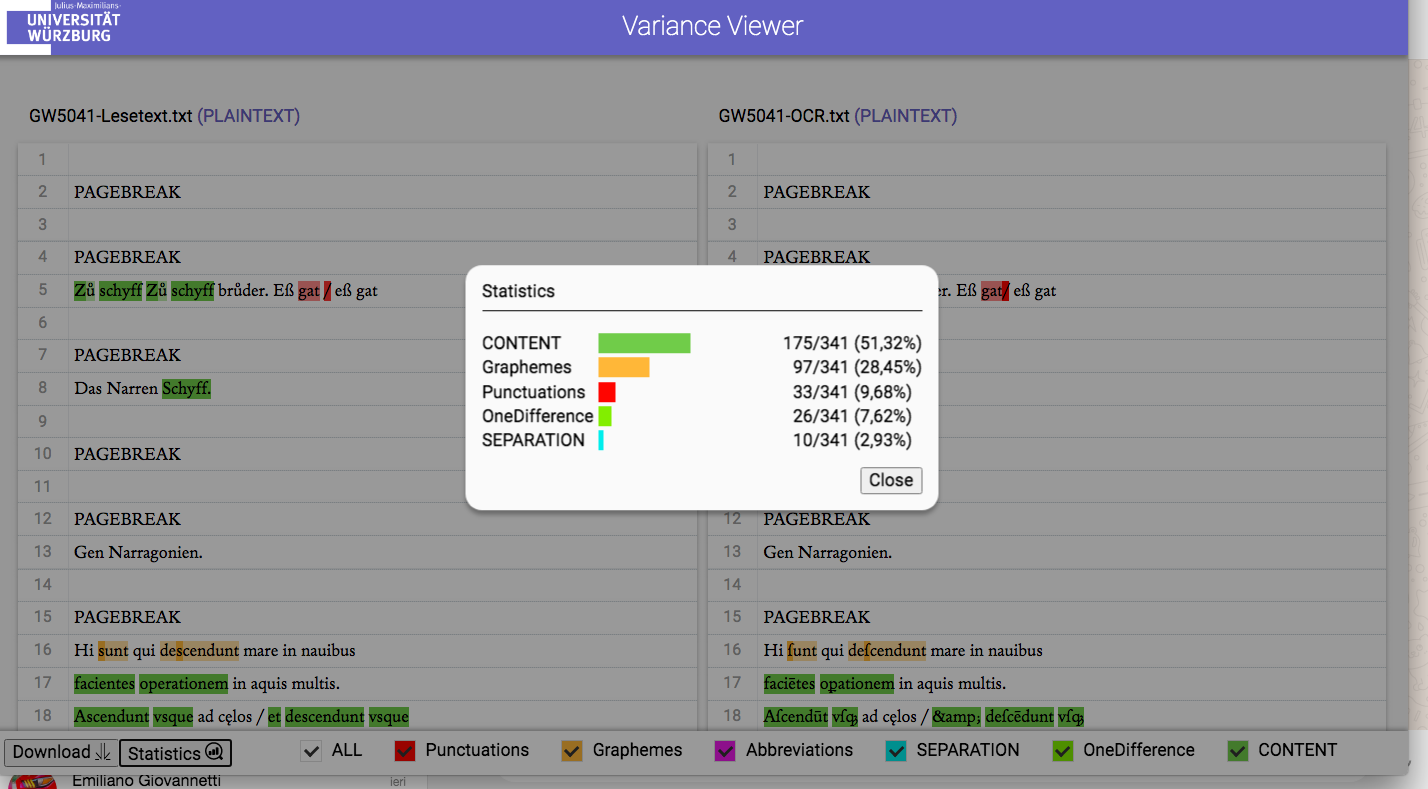
\includegraphics[width=.95\textwidth]{imgs/variance-viewer.png}
	\end{center}
\end{frame}

\begin{frame}
    \frametitle{Strumenti per edizioni critiche}
    \framesubtitle{Strumenti di collazione automatica}
	\addtocounter{nframe}{1}
    \begin{center}
        \textbf{Juxta Web Service}
    \end{center}
    \begin{center}
        \textit{\url{http://juxtacommons.org/}}
	\end{center}
    \begin{center}
        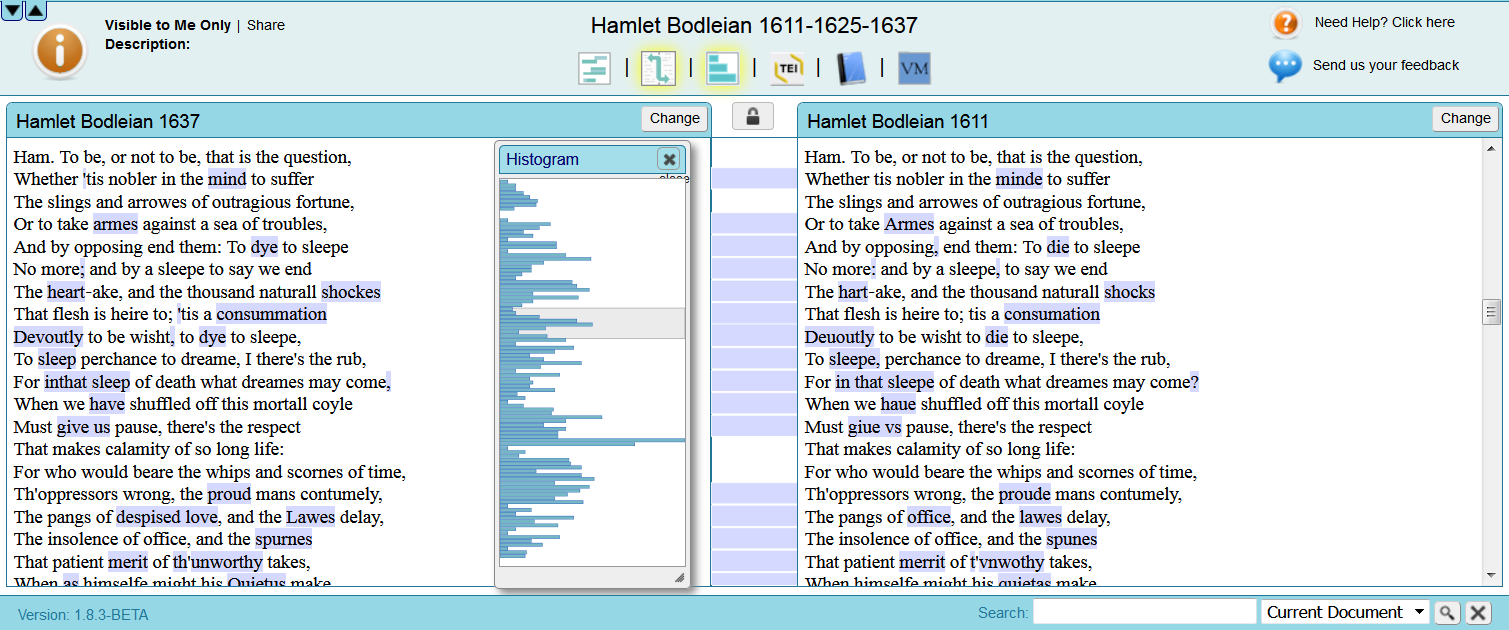
\includegraphics[width=.95\textwidth]{imgs/juxtaweb.png}
	\end{center}
\end{frame}

\begin{frame}
    \frametitle{Strumenti per edizioni critiche}
    \framesubtitle{Strumenti di collazione automatica}
	\addtocounter{nframe}{1}
    \begin{center}
        \textbf{StemmaWeb}
    \end{center}
    \begin{center}
        \textit{\url{https://stemmaweb.net/stemmaweb/}}
	\end{center}
    \begin{center}
        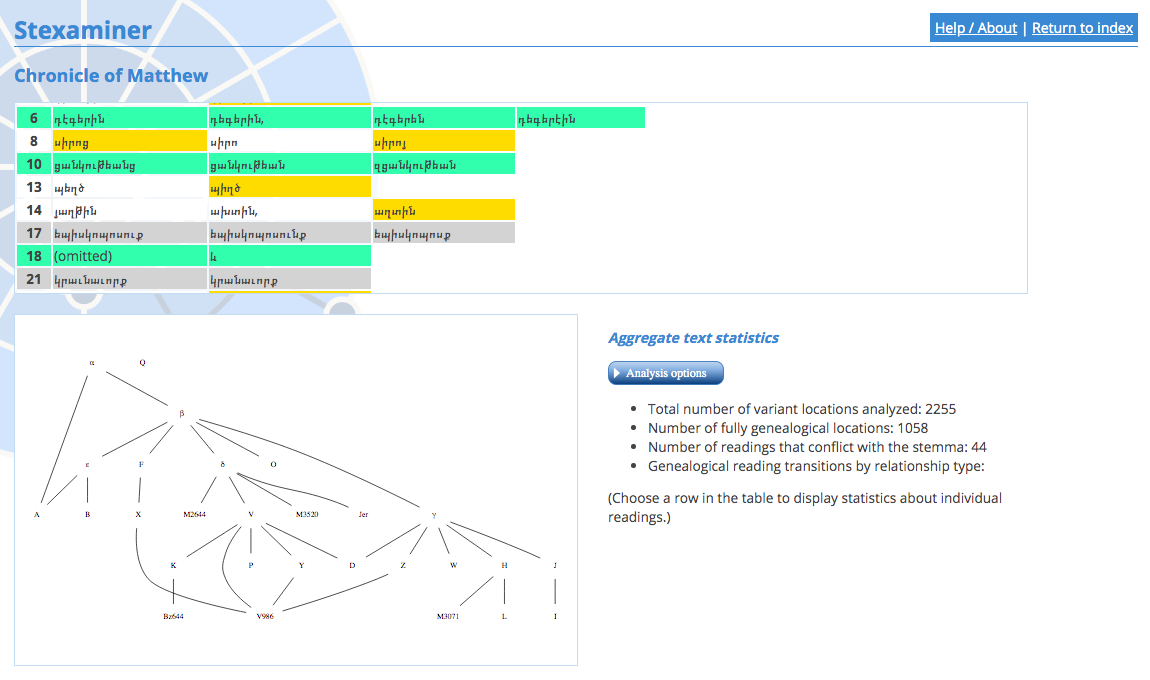
\includegraphics[width=.95\textwidth]{imgs/stemmaweb.png}
	\end{center}
\end{frame}

\begin{frame}
    \frametitle{Strumenti per edizioni critiche}
    \framesubtitle{Strumenti di collazione automatica}
	\addtocounter{nframe}{1}
    \begin{center}
        \textbf{TUebingen System of Text Processing Programs" TUSTEP - TXSTEP}
    \end{center}
    \begin{center}
        \textit{\url{https://www.tustep.uni-tuebingen.de/tustep_eng.html}}
	\end{center}
    \begin{center}
        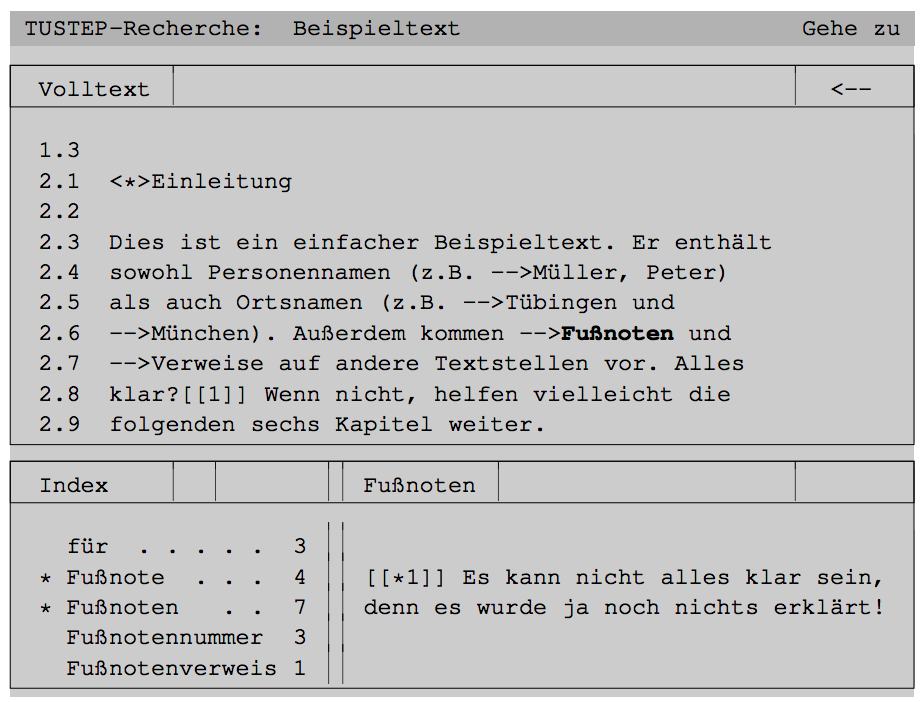
\includegraphics[width=.95\textwidth]{imgs/tustep.png}
	\end{center}
\end{frame}

\begin{frame}
    \frametitle{Strumenti per edizioni critiche}
    \framesubtitle{Strumenti di collazione automatica}
	\addtocounter{nframe}{1}
    \begin{center}
        \textbf{MEDITE}
    \end{center}
    \begin{center}
        \textit{\url{http://www-poleia.lip6.fr/~ganascia/Medite\_Project}}
	\end{center}
    \begin{center}
        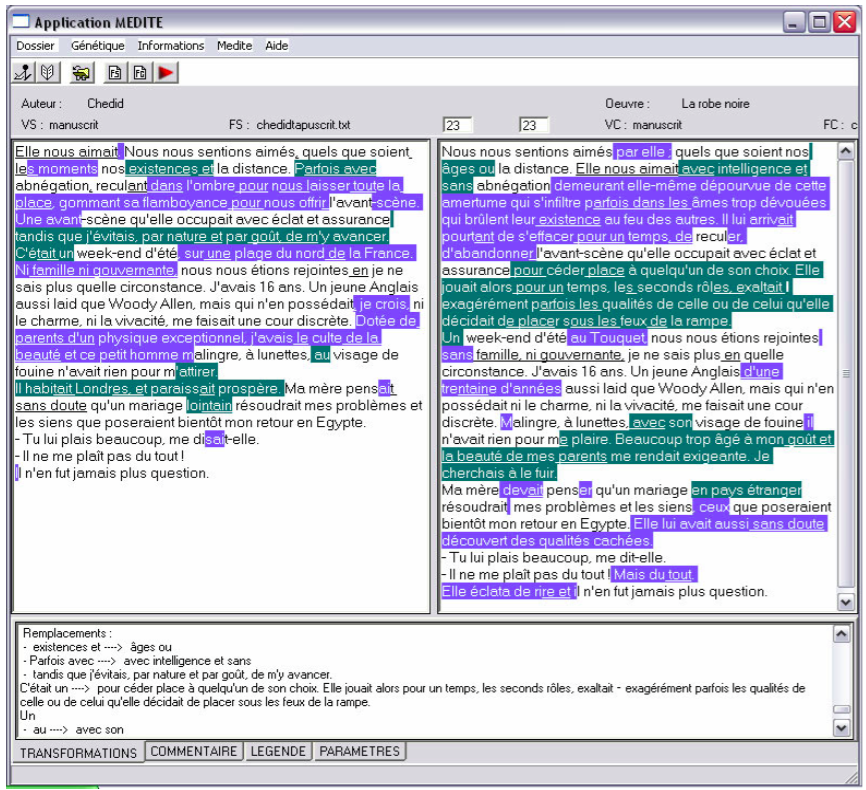
\includegraphics[width=.95\textwidth]{imgs/medite.png}
	\end{center}
\end{frame}


\begin{frame}
    \frametitle{Strumenti per edizioni critiche}
    \framesubtitle{Strumenti per la visualizzazione e pubblicazione}
	\addtocounter{nframe}{1}
    \begin{center}
        \textbf{Classical Text Editor}
    \end{center}
    \begin{center}
        \textit{\url{https://cte.oeaw.ac.at/}}
	\end{center}
    \begin{center}
        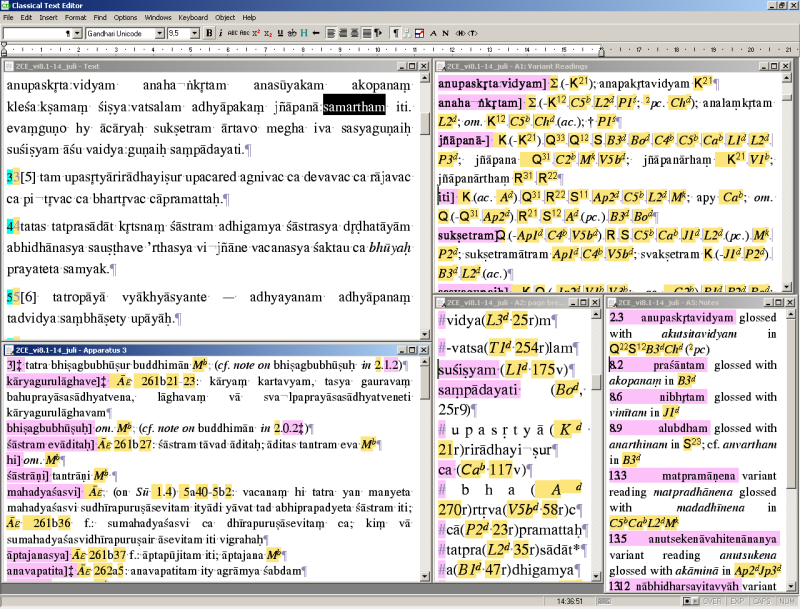
\includegraphics[width=.95\textwidth]{imgs/cte.png}
	\end{center}
\end{frame}

\begin{frame}
    \frametitle{Strumenti per edizioni critiche}
    \framesubtitle{Strumenti per la visualizzazione e pubblicazione}
	\addtocounter{nframe}{1}
    \begin{center}
        \textbf{TEIpublisher}
    \end{center}
    \begin{center}
        \textit{\url{https://teipublisher.com/index.html}}
	\end{center}
    \begin{center}
        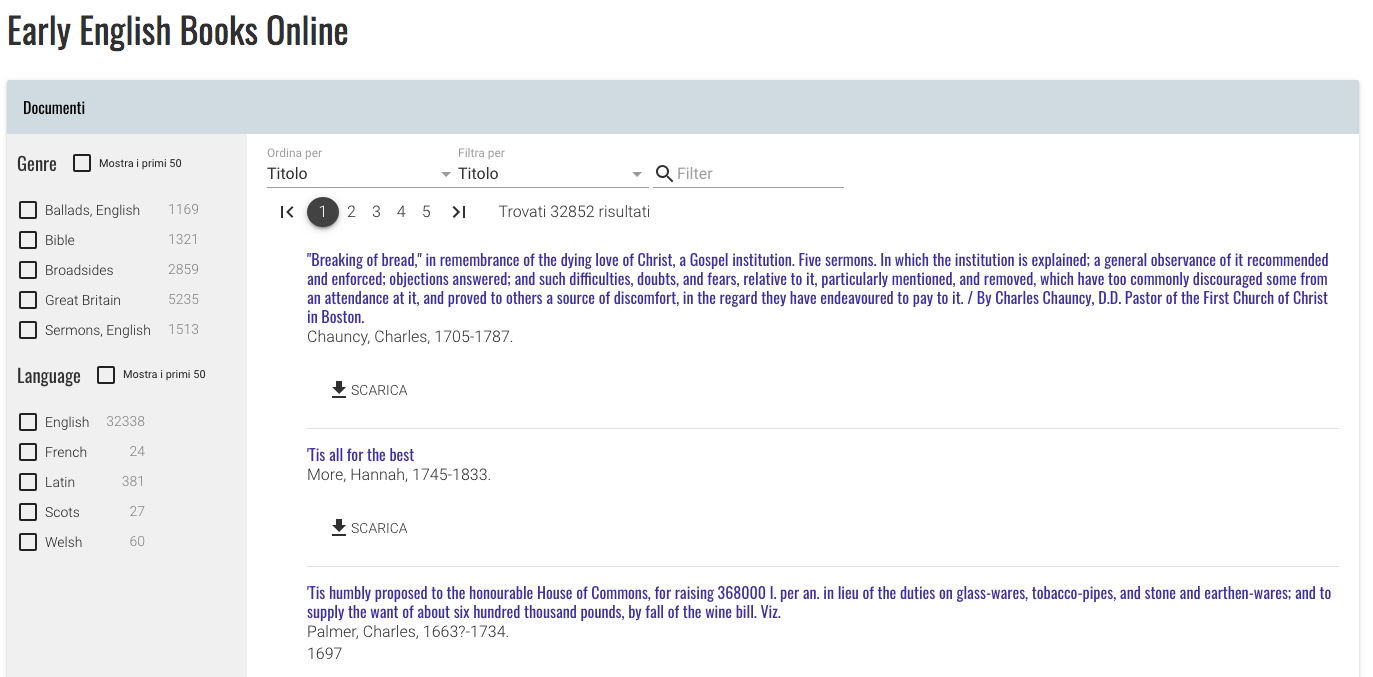
\includegraphics[width=.95\textwidth]{imgs/teipublisher.png}
	\end{center}
\end{frame}

\begin{frame}
    \frametitle{Strumenti per edizioni critiche}
    \framesubtitle{Strumenti per la visualizzazione e pubblicazione}
	\addtocounter{nframe}{1}
    \begin{center}
        \textbf{Edition Visualization Technology (EVT)}
    \end{center}
    \begin{center}
        \textit{\url{http://evt.labcd.unipi.it}}
	\end{center}
    \begin{center}
        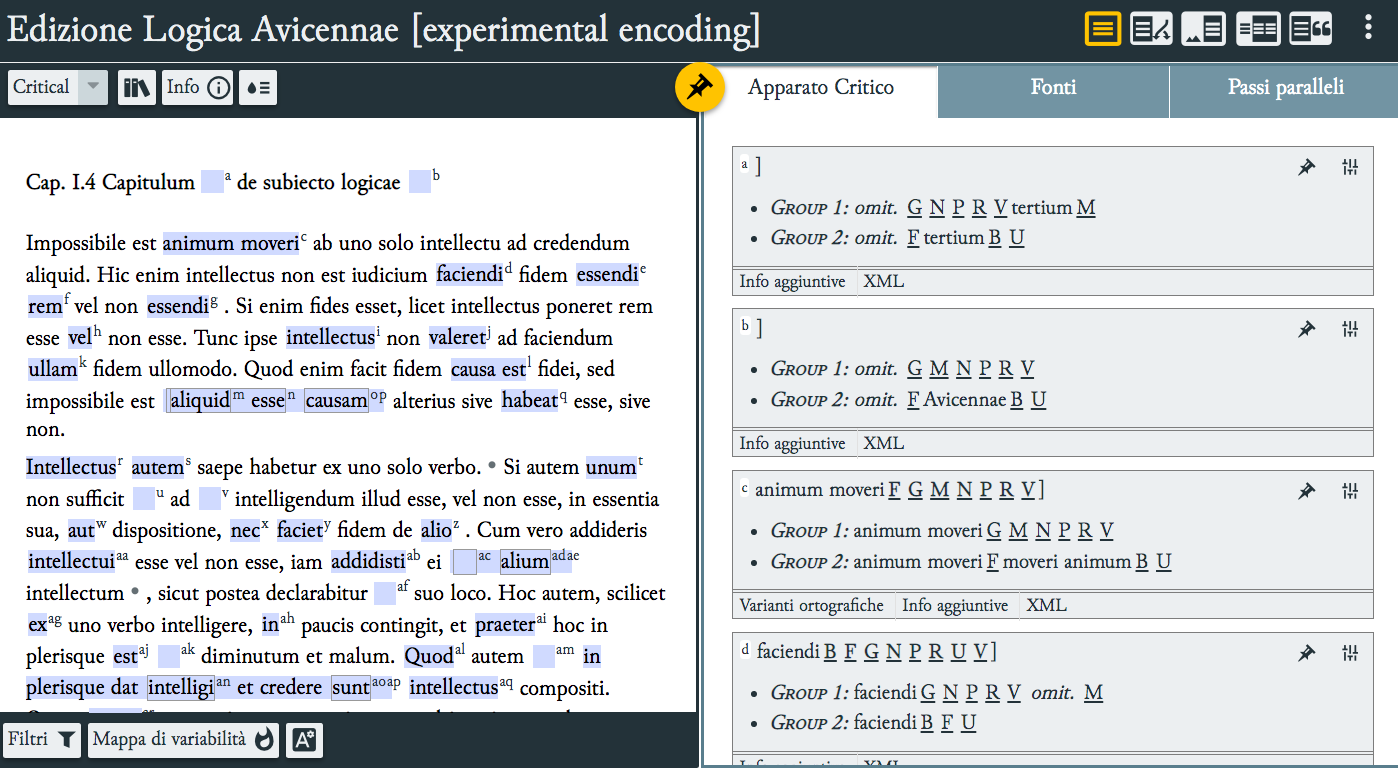
\includegraphics[width=.95\textwidth]{imgs/evt.png}
	\end{center}
\end{frame}

\begin{frame}
    \frametitle{Strumenti per edizioni critiche}
    \framesubtitle{Strumenti per la visualizzazione e pubblicazione}
	\addtocounter{nframe}{1}
    \begin{center}
        \textbf{Textual Communities}
    \end{center}
    \begin{center}
        \textit{\url{https://textualcommunities.org/app/}}
	\end{center}
    \begin{center}
        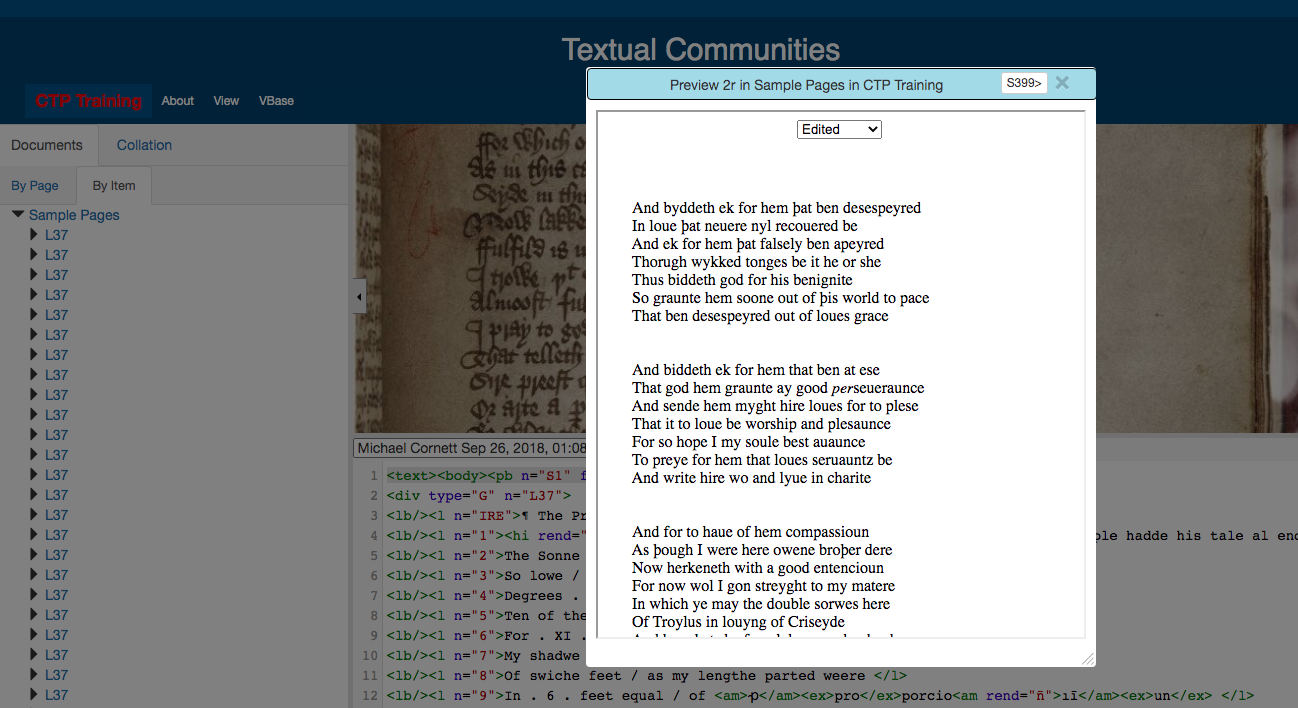
\includegraphics[width=.95\textwidth]{imgs/textualcommunities.png}
        
	\end{center}
\end{frame}

\begin{frame}
    \frametitle{Strumenti per edizioni critiche}
    \framesubtitle{Strumenti per la visualizzazione e pubblicazione}
	\addtocounter{nframe}{1}
    \begin{center}
        \textbf{Versioning Machine}
    \end{center}
    \begin{center}
        \textit{\url{http://v-machine.org}}
	\end{center}
    \begin{center}
        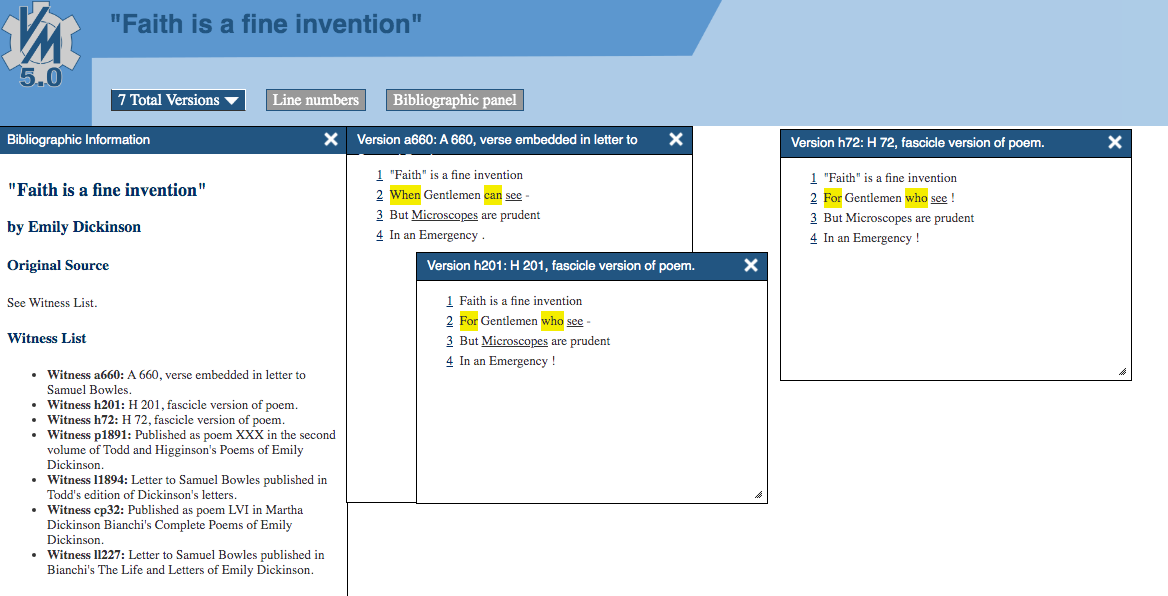
\includegraphics[width=.95\textwidth]{imgs/v-machine.png}
	\end{center}
\end{frame}

\begin{frame}
    \frametitle{Strumenti per edizioni critiche}
    \framesubtitle{Strumenti per la visualizzazione e pubblicazione}
	\addtocounter{nframe}{1}
    \begin{center}
        \textbf{LERA/SADA project}
    \end{center}
    \begin{center}
        \textit{\url{https://sada.uzi.uni-halle.de/}}
	\end{center}
    \begin{center}
        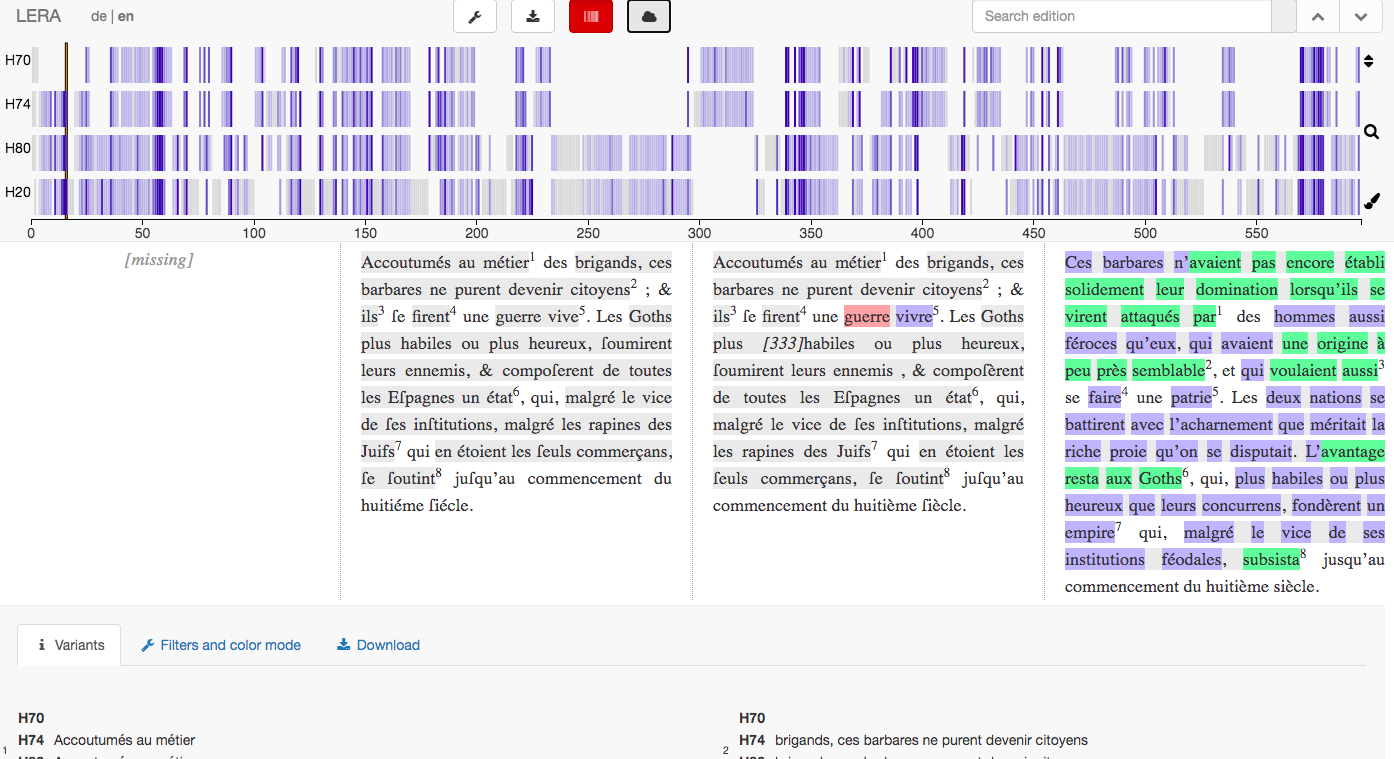
\includegraphics[width=.95\textwidth]{imgs/lara.png}
	\end{center}
\end{frame}

\begin{frame}
    \frametitle{Strumenti per edizioni critiche}
    \framesubtitle{Strumenti per la visualizzazione e pubblicazione}
	\addtocounter{nframe}{1}
    \begin{center}
        \textbf{Critical Edition Toolbox}
    \end{center}
    \begin{center}
        \textit{\url{http://teicat.huma-num.fr/index.php}}
	\end{center}
    \begin{center}
        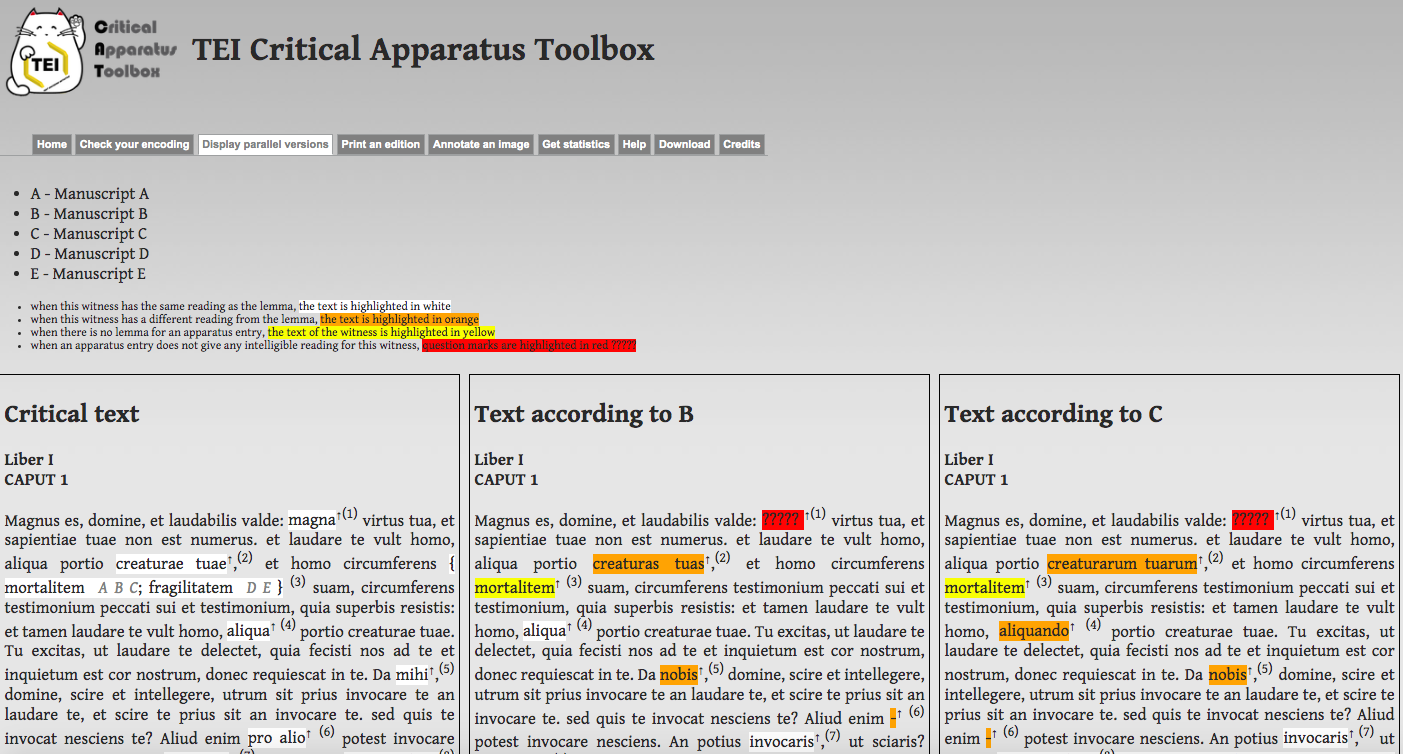
\includegraphics[width=.95\textwidth]{imgs/TEI-critical-app-toolbox.png}
	\end{center}
\end{frame}

\begin{frame}
    \frametitle{Strumenti per edizioni critiche}
    \framesubtitle{Strumenti per la visualizzazione e pubblicazione}
	\addtocounter{nframe}{1}
    \begin{center}
        \textbf{LaTex/Reledmac}
    \end{center}
    \begin{center}
        \textit{\url{https://ctan.org/pkg/reledmac}}
	\end{center}
    \begin{center}
        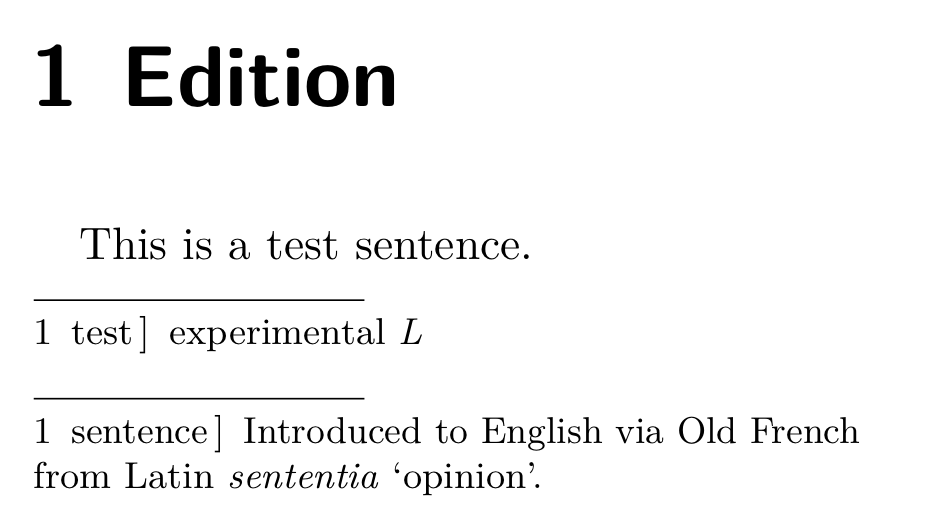
\includegraphics[width=.95\textwidth]{imgs/reledmac-test.png}
	\end{center}
\end{frame}

\begin{frame}
    \frametitle{Strumenti per edizioni critiche}
    \framesubtitle{Strumenti per la visualizzazione e pubblicazione}
	\addtocounter{nframe}{1}
    \begin{center}
        \textbf{TRAVIZ/ITEAL}
    \end{center}
    \begin{center}
        \textit{\url{http://www.traviz.vizcovery.org/}}
	\end{center}
    \begin{center}
        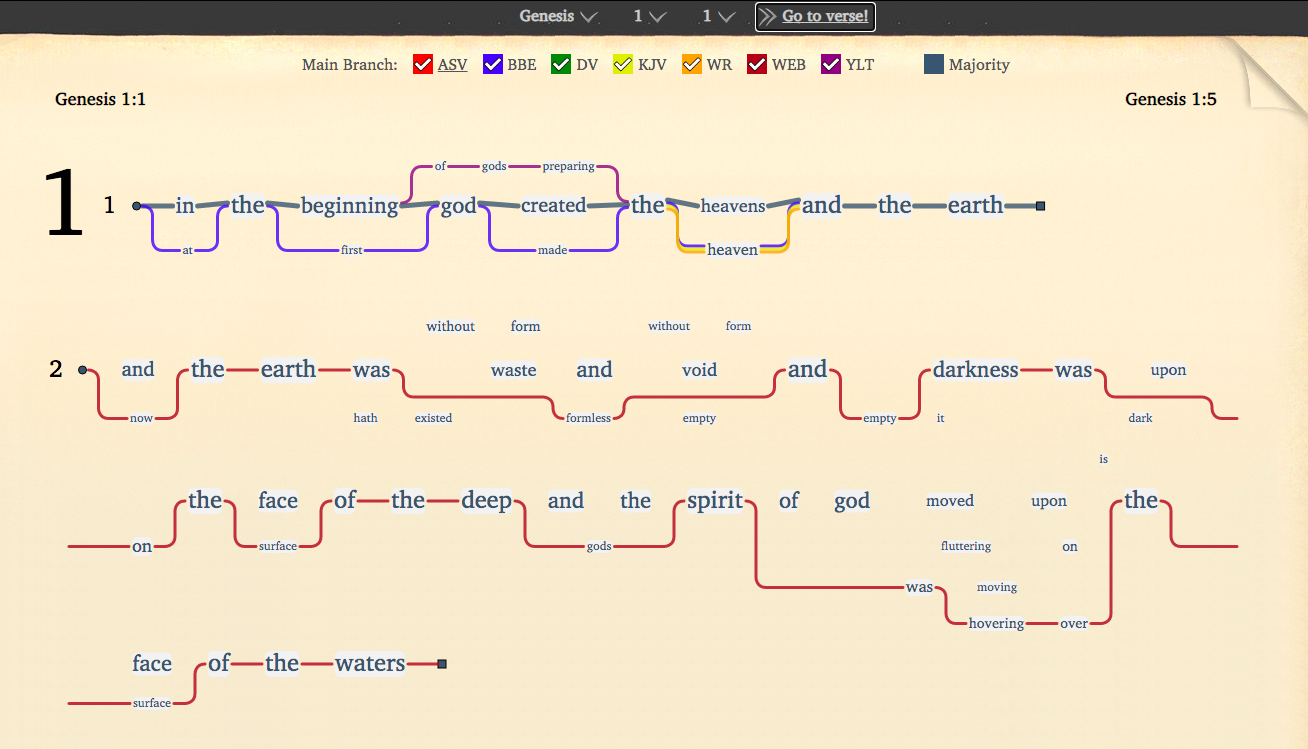
\includegraphics[width=.95\textwidth]{imgs/traviz.png}
	\end{center}
\end{frame}

\begin{frame}
    \frametitle{Strumenti per edizioni critiche}
    \framesubtitle{Strumenti per la visualizzazione e pubblicazione}
    \addtocounter{nframe}{1}
    
    \begin{center}
        \textbf{EUPORIA}
    \end{center}
    \begin{center}
        \textit{\url{cophilab.ilc.cnr.it}}
    \end{center}
    
    \begin{center}
        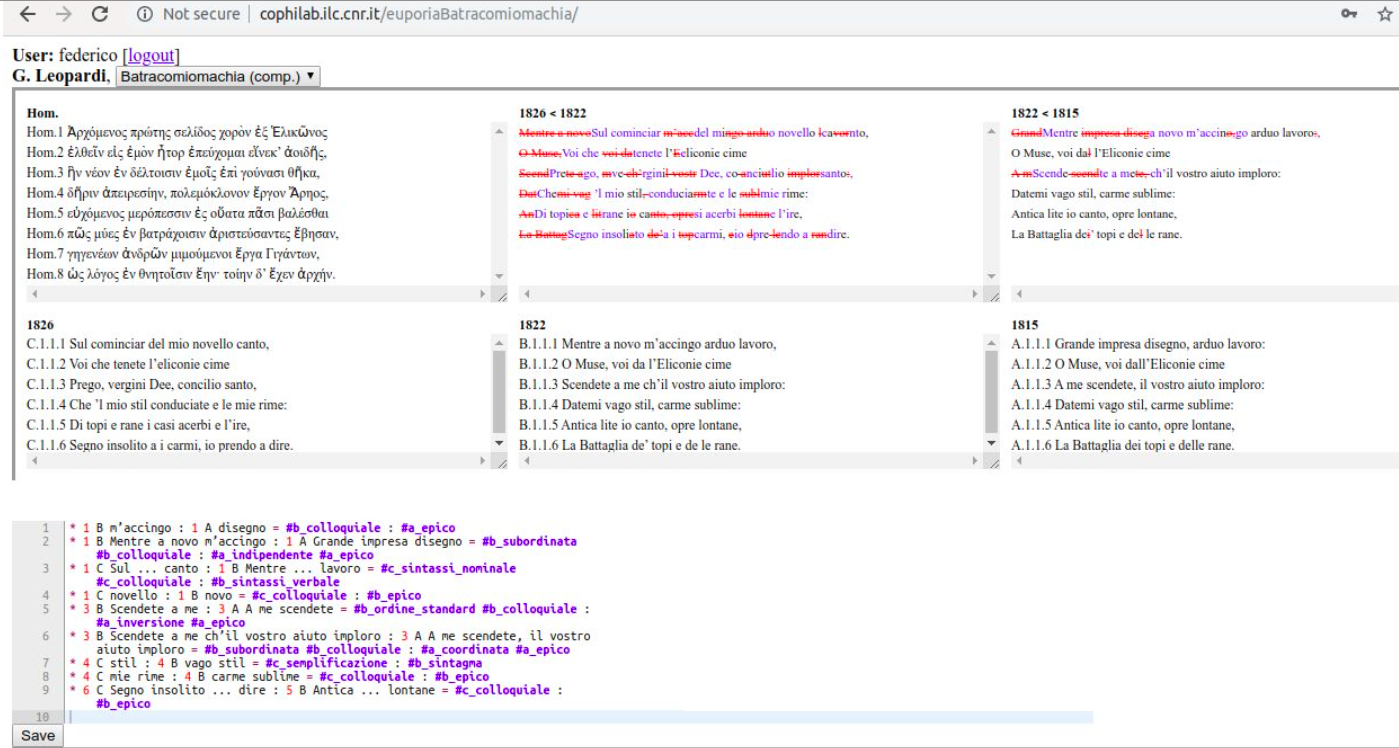
\includegraphics[width=.95\textwidth]{imgs/euporia.png}
	\end{center}
\end{frame}

